\chapter{INTRODUCTION}
\pagenumbering{arabic}

\section{Overview}
The current progress in computer vision (V) and natural language processing (L) is inspiring. Representative V+L tasks include visual question answering (VQA), image/video captioning, textual grounding system, and image/video retrieval by language tasks. All these tasks have significant meanings to real-world applications: VQA and captioning systems can be the ground of cross-modal conversation systems, VL retrieval might be helpful for next-generation searching engines, and the textual grounding system helps to localize certain objects by open-form, and human-readable natural languages in robotics.


\begin{figure}
\begin{center}
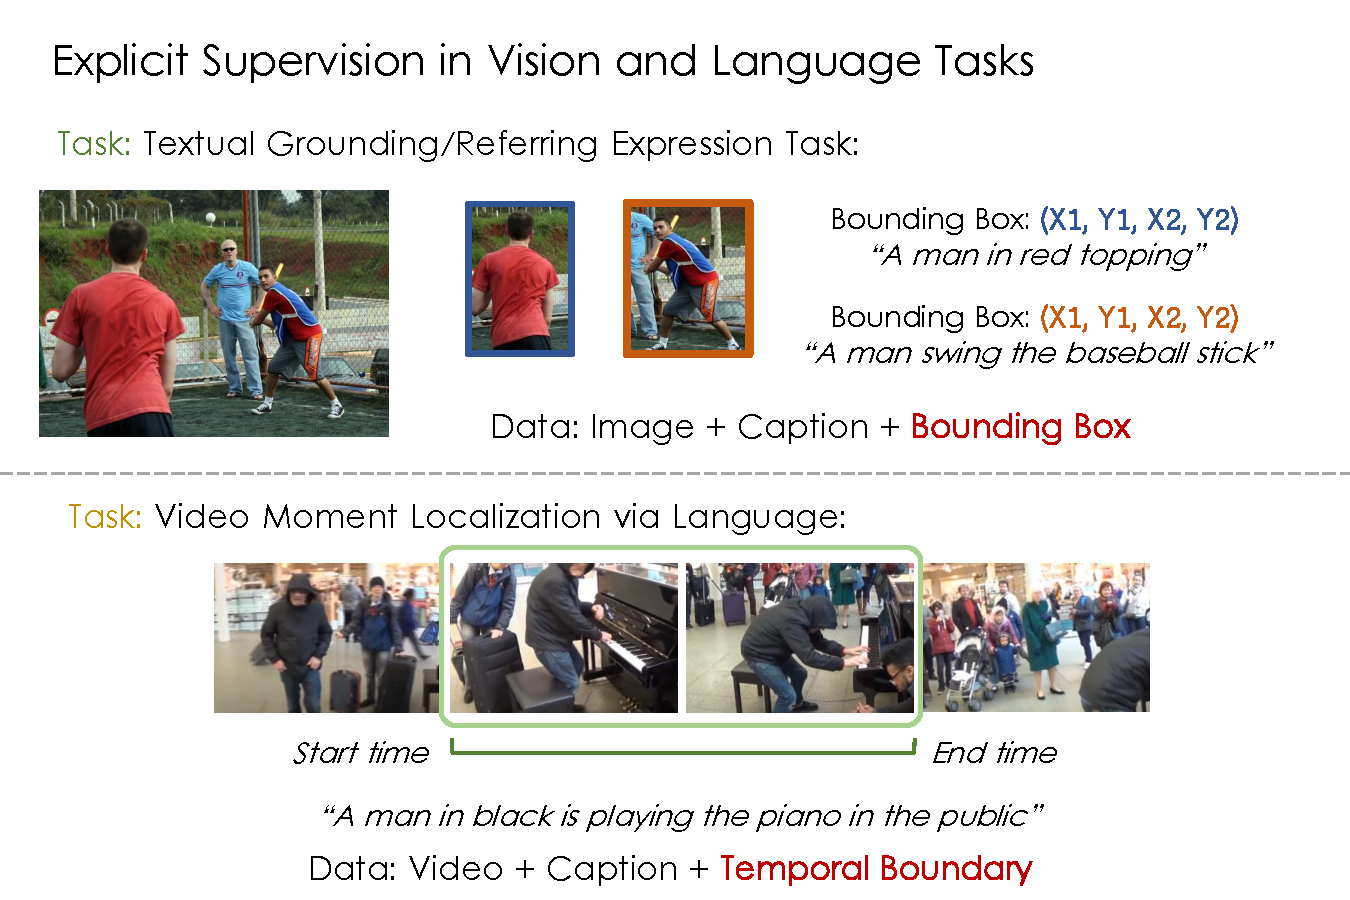
\includegraphics[width=.99\textwidth]{images/explicit_training.pdf}
\end{center}
\caption[Example of some VL tasks.]{VL tasks like textual grounding, referring expression and video moment localization via language unanimously require explicit annotations (\ie, bounding boxes of target objects or temporal boundaries for the moments) for learning of visual-textual correlation.
}
\label{fig:explicit_learning}
\end{figure}

Despite these, there exist several critical challenges that prevent us from pushing these advances to the real world.  One of the most difficult problems comes from the prohibitively expensive human labeling: previous powerful VL models are mostly domain-specific that rely heavily on a well-annotated VL dataset by humans, \eg, image captioning dataset like COCO~\citep{lin2014microsoft} collected  328K images, covering image-level object annotations and also captions explaining the content of images. Beyond that, the development of powerful VL systems like textual grounding models requires the awareness of spatial location per object (see Figure~\ref{fig:explicit_learning} for example). Compared with the countless images the system might encounter in the real world, annotating images at scale in COCO-style is hardly practical, nor financially effective. This spawns the challenge for the VL community: how to train a unified VL model that can be transferred to diverse domains via the implicit supervisions (\ie, large volume of weakly-annotated, or even un-labeled raw visual+textual data). Unlike the traditional vision model (object detection or recognition model), the VL model usually requires the understanding of correlations between visual concepts with rich semantics, while the traditional visual model only performs on a bunch of pre-defined and limited categories.


Another notable challenge arises when deploying the VL model on an edge device that usually has the limited computational power to be undertaken. It is impractical for real-world applications to exploit the power of prevailing VL models under a constrained training/inference budget due to their cumbersome sizes and huge computation cost. Building a lightweight VL model, meanwhile improving its performances is of great practical value but is less explored in the previous literature. In the furtherance of gaining a more real-world practical compact VL model, we study to exploit knowledge distillation techniques to improve the VL representation learning on compact models. 


Following the above-mentioned, I work on making contributions in the following aspects:

\begin{figure}
\begin{center}
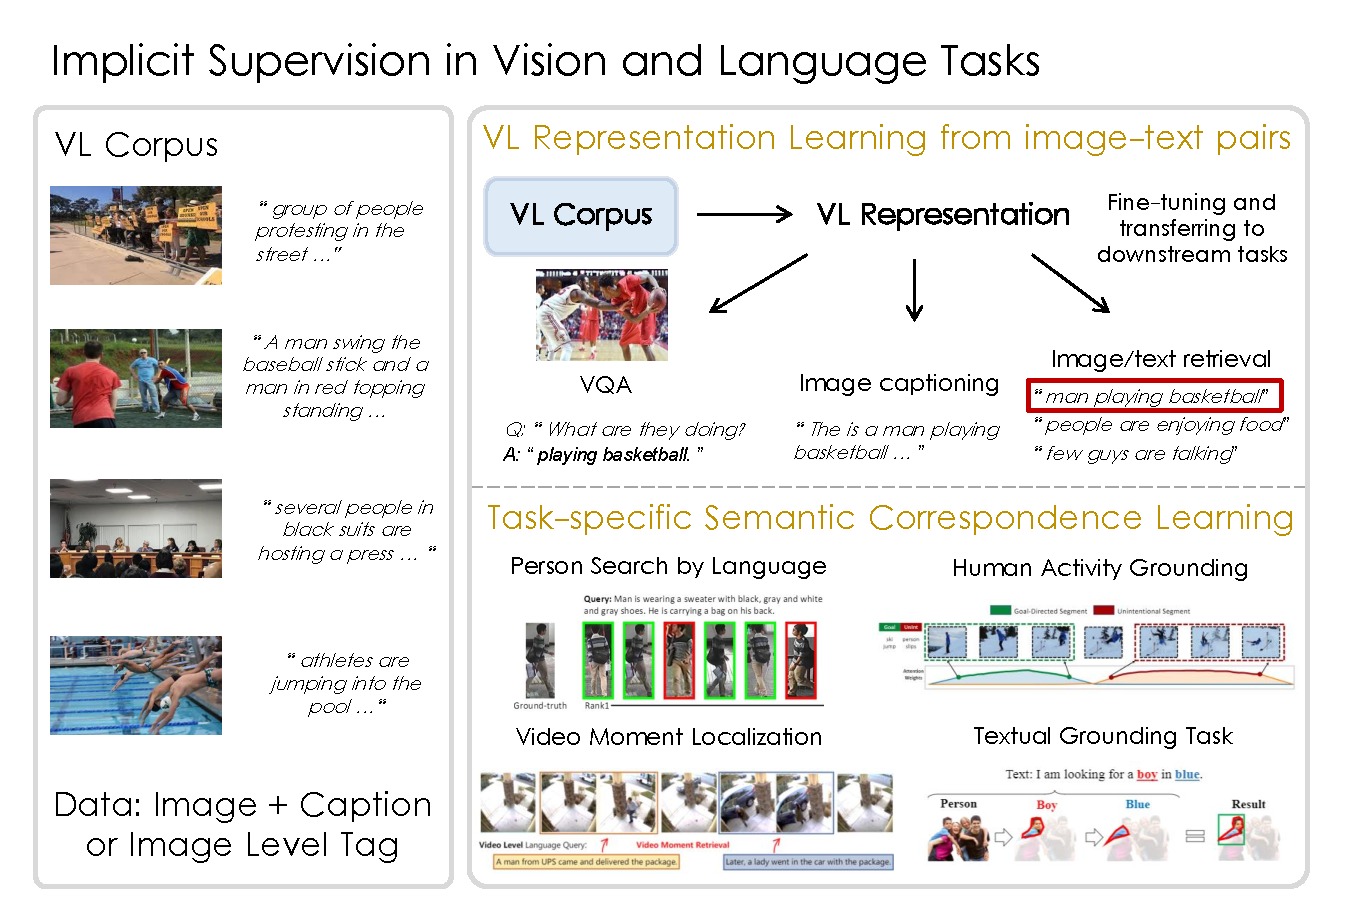
\includegraphics[width=.99\textwidth]{images/implicit_training.pdf}
\end{center}
\caption[VL Representation Learning \vs Downstream VL tasks.]{Unlike explicit VL supervisions, the training on implicit VL supervisions aims to learn either 1). task-agnostic and generic VL representations that can be transferred to other VL tasks, or 2). specific VL task (\eg, grounding, retrieval, etc). The former task focuses more on how to learn the VL representations from image-text pairs with better generalization and expressive semantics when there is no explicit training objective, while the latter requires a task-specific learning method (\eg, multi-instance learning).
}
\label{fig:implicit_learning}
\end{figure}

1. Learn the associations between visual concepts and semantics in a weak/un-supervised fashion. For example, when given an image, learn which specific region best corresponds to a textual query ``\textit{A man in red topping}'', when we have only an image-level general description like ``\textit{A man swing the base ball stick and a man in red topping standing in the playground ...}'', without knowing the exact region corresponds to specific visual concepts (a.k.a, weakly-supervised textual grounding in images/videos).

2. Learn ``omni''-VL representations that can be transferred to diverse VL tasks from image-text pairs via pre-training and fine-tune fashion. Now as the VL pre-training leverages only general image+text pairs without further spatial, or pixel-level annotations, it is challenging how to effectively mine the hidden visual-textual associations at scale for representation learning (as is shown in Figure~\ref{fig:implicit_learning}). Beyond that. I also work on leveraging task-agnostic knowledge distillation in assisting the representation learning on small and generic VL models. 

3. Build an efficient VL model. Much of the existing VL models focus on large models that suffer from high latency and large memory footprints at the time of inference, which limits their deployment to resource-constrained edge devices for real-world applications. I study how to train small and efficient VL models from the perspective of Knowledge Distillation for model compression. In the end, I explain the feasibility of developing the ``one-stage VL model'' which does not require the cumbersome object detector and thus brings obvious flexibility for both model training and inference. 

% Figure~\ref{fig:explicit_learning} gives an overview of the major aspects of this dissertation. 
This dissertation highlights a few selected research projects I worked on from the aforementioned perspective: 1). A textual grounding system that learns the semantic correspondence from weakly supervised learning~\citep{Fang_2019_CVPR,fang2019temporal}. 2). A novel self-supervised visual representation learning paradigm coupled with knowledge distillation~\citep{fang2020seed}. 3). A compact VL model that benefits from VL distillation, which can be transferred to a series of other generic downstream VL tasks~\citep{fang2021compressing}. Also an one-stage image captioning model that brings training flexibility and inference speed~\citep{fang2021injecting}. All of these efforts reflect my primary research in the intersection of computer vision and natural language processing that advances the V+L learning from implicit supervisions with increased efficiency.

\section{Preliminaries}
To give the readers a more comprehensive background introduction about the Vision and Language and some relevant techniques this dissertation mentions later, I will briefly review several Vision Language tasks, together with their formulation under the weakly-supervised learning schema. These weakly-supervised VL tasks are less data-dependent than they attempt to learn the cross-modal correspondence without explicit supervision. Nevertheless, they are inevitably limited to only specific VL tasks that need manual design. To circumvent these, a broader series of works alter to introduce the generic representation learning from a large VL corpus that their ``omni''-representations are transferable to different downstream tasks and are entirely task-agnostic during the pre-training phase.

\subsection{Glance of Prevailing VL Tasks}


\begin{figure}
\begin{center}
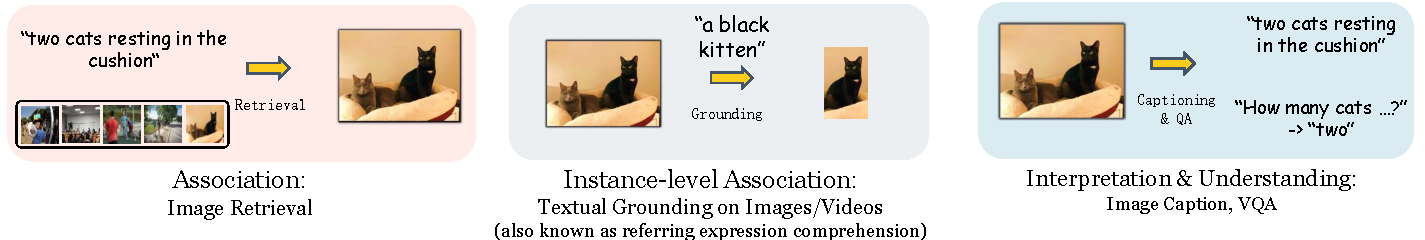
\includegraphics[width=.99\textwidth]{images/VL-tasks.pdf}
\end{center}
\caption[Prevailing VL Tasks.]{Glance of some representative VL tasks from different perspectives. The image content retrieval task builds upon the association relationship across the Vision and Language modalities. Proceeding from that, this association extends to the instance-level that one can retrieve either a region of the image covering a specific object or a short video moment containing an event in untrimmed video. High-level VL tasks involve more interpretation and understanding: for instance, generating a textual description from the observation, or answering the question based on the visual observation.}
\label{fig:VLtasks}
\end{figure}

\noindent{\bf Association Learning across Vision and Language} is core and tie of a wide range of tasks across vision and language domains, \emph{e.g.}, textual grounding~\citep{plummer2015flickr30k}, referring expression comprehension~\citep{nagaraja2016modeling} or object retrieval using language~\citep{hu2016natural}. In particular, given an image $\mathbf{I}$, {T}extual {G}rounding model selects a proposal $\mathbf{c}$ given a textual query $\mathbf{T}$ from a set of coordinates $\mathbf{C} = \{\mathbf{c_1 \dots c_N}\}$ (see example in Figure~\ref{fig:VLtasks}):
\begin{equation}
    \mathbf{c} = \text{Textual-Grounder}{\big(}\mathbf{I}, \mathbf{T},\mathbf{C}{\big)},
\end{equation}
where $N$ denotes the number of candidate proposals generated by some generic proposal network. To obtain a strong textual grounding model, one might need to collect massive \texttt{<image-text-proposal>} triplets to sufficiently train such a model. 
Such association learning also extends to the video domains ({V}ideo {L}ocalization Task) where the textual description is utilized as the query to anchor a clip from a long untrimmed video:
\begin{equation}
    \mathbf{c} = \text{Moment-Localizer}{\big(}\mathbf{V}, \mathbf{T}, \mathbf{C}{\big)},
\end{equation}
where now the proposal $\mathbf{c}$ is selected as the temporal boundary of a video moment with starting time $t_s$ and ending time $t_e$ of the video $\mathbf{V}$.

Recent works shed light on the importance of leveraging the image-level annotations (as weak supervision)~\citep{fang2018modularizedtextual,fang2018weakly} or unsupervised method~\citep{yeh2018unsupervised} to learn the association across language descriptions and objects. Proceeding from this, there arise works on using uncurated captions to learn temporal associations across video segments and texts~\citep{miech2019end,sun2019videobert}. Notably, these works all highlight the importance of constructing contrastive pairs in exploiting the weak annotations. We will discuss more about the contrastive learning at later section. 

\noindent{\bf Visual Interpretation via Language} tasks laid more emphasis on the high-level understanding aspects. Typical interpretation tasks include \emph{Visual Captioning} and \emph{Visual Question Answering} Tasks (an example is shown in Figure~\ref{fig:VLtasks}). Visual captioning is perhaps the first step towards understanding images/videos and describing their content in natural language.
Recent advances in visual captioning have been able to generate captions that describe humans and objects and their interactions in the video.
They seek to generate paragraphs or multi-sentence captions about the content of images or videos.
It is important to note that visual captioning systems have a major limitation in that they can only generate factual descriptions about observable objects or events in the video yet without full \emph{understanding} the content. For detailed visual understanding, we would like to go beyond observable visual entities and use background knowledge and contextualization to reason about the observation and answer the questions. Most existing VQA benchmarks only predict answers from a pre-constructed \& limited answer sets, largely limits the practical scopes of the systems. Few recent works propose the open-domain VQA task~\citep{chang2021webqa} that generates the answers directly, or the VQA tasks need external knowledge~\citep{wang2017fvqa,zellers2019vcr,marino2019ok,garcia2020knowit,7298682}


\subsection{Implicit Supervisions for VL Tasks}
\noindent{\bf Weakly Supervised Learning} receives increasing attention~\citep{deselaers2010localizing,pandey2011scene, cinbis2017weakly,mahajan2018exploring,pathak2015constrained,pinheiro2015image,xu2014tell}.
It focuses on learning granular detectors given only coarse annotations.
This is of practical significance as granular annotations (\eg, bounding boxes and pixel-level labels) are much more expensive to obtain compared to coarse image-level annotations.
Recent studies show that weakly supervised methods can even outperform the strongly supervised method for image classification~\citep{mahajan2018exploring,ge2019weakly},
and is even widen to a wide range of vision tasks, including object detection~\citep{bilen2014weakly,shen2018generative,bilen2016weakly}, semantic segmentation~\citep{kervadec2019constrained,pathak2015constrained,wei2016stc} and etc.
In video analysis domain, the weakly-supervised action localization is frequently studied and can be thought of a specific example of learning with the video-level labels~\citep{sun2015temporal,shou2018autoloc,nguyen2018weakly,paul2018w}.
This problem derives from the fully-supervised counterpart methods which exploits fine annotations at frame level
for localizing the actions~\citep{buch2017sst,kalogeiton2017action,weinzaepfel2015learning,shou2017cdc,tran2012max,shou2016temporal}.
Recent weakly-supervised methods extensively adopt either the video-level classification framework~\citep{singh2017hide,shou2018autoloc,sikka2014classification,dwibedi2019temporal} or with the attentional mechanism 
that generates bottom-up sparse weights used for localizing action categories temporally~\citep{nguyen2018weakly}. Beyond that, few works~\citep{wang2017untrimmednets,paul2018w} propose to utilize the multi-instance learning loss to address this challenge,~\citep{paul2018w} also suggests exploiting the co-activity across videos in the metric learning, which largely improves the action localization task even when temporal annotations are not available. The most recent work~\citep{nguyen2019weakly} improves over these methods with a background modeling module that explicitly extracts the foreground and background appearances.  This dissertation focus more on extending this weakly supervised learning signals to VL tasks.\footnote{Implicit supervisions in this dissertation refer to both weakly-supervised learning and self-supervised learning.}

% Unlike current work,
% we perform weakly-supervised learning for textual grounding, including training for both entity grounding
% and textual-visual matching through a progressive modular procedure.

% Modular design is also receiving more attention recently, mainly for
% complex systems like visual-question-answering or image captioning~\citep{hu2017modeling, hu2018explainable,
% yu2018mattnet}.
% Such modular design is carried out by realizing some linguistic structures.
% In our work,
% we propose to decompose the query textual description into progressive levels,
% each of which is passed to a corresponding module,
% and then produce the final grounding result by progressively merging the intermediate results.
% In this way,
% our system enjoys high interpretability and resilience to counterfactual inputs.

% Few works also shed light upon the importance of contrastive learning for weak supervision.


\noindent{\bf Weakly-Supervised Image/Video Grounding by Language} 
We are concerned with the model's dependency on the complicated data annotations for textual grounding task. For this reason, it is important to study how to build 

Temporal Grounding and Moments Retrieval are two instantiations of learning
temporal-textual association.
In these tasks, most recent methods adopt fully-supervised training over 
fine annotations on the frame-textual associations.
For example, Gao \emph{et al.} augment the Charades 
dataset~\citep{sigurdsson2016hollywood} by generating complex language queries with temporal boundary annotations for language moment retrieval~\citep{gao2017tall}; 
Anne Hendricks \emph{et al.} also collect a new dataset for training to localize video moments over a given descriptive sentence~\citep{anne2017localizing}. 
Other follow-up methods~\citep{hendricks2018localizing,liu2018attentive,chen2018temporally,wang2018bidirectional,xu2019joint,gavrilyuk2018actor} also
fully-supervised train for temporal grounding using these datasets,
suffering from the limitation on their generalizability due to  
the combinatorial nature of complex natural language sentences (\textit{e.g.}, 
synonymous words, grammatical tense 
and sentence structures)~\citep{hendricks2018localizing,gao2017tall}. 
advances the aforementioned to an even challenging task, as now the only available supervision is video-level natural language descriptions in an open format, which come with a huge amount of unnecessary noises.
In particular, Mithun \emph{et al.}~\citep{Mithun_2019_CVPR} for the first time attempted to 
solve the temporal grounding problem by weakly supervising learning 
with only the video-level textual queries~\citep{Mithun_2019_CVPR}. 
In~\citep{chen2020look}, the author proposed to utilize the temporal proposal and textual description alignment learning using the sliding window fashion and tackle the grounding problem in a coarse-to-fine manner. Similarly, a very recent work by~\citep{lin2019weakly} also focuses on the design of a better proposal generation module, that aggregates the contextual visual cues to generate and score the proposed candidates for grounding. We summarize that current efforts in weakly supervised language grounding are either centered on better proposal generation~\citep{chen2020look,lin2019weakly} or a better cross-modal association model by constructing contrastive samples across video and languages~\citep{Mithun_2019_CVPR,gao2019wslln}. Our WSRA (introduced in later Chapter) places emphasis on the latter, but nevertheless further distinguishes the above with a more comprehensive cross-modal association learning objectiveness and a novel sampling and weighting strategy in our metric learning step.

\subsection{VL Representation Learning from Weak Annotations}

Following the prominent progress in the transformer-based (introduced in later section)~\citep{vaswani2017attention} pre-training in natural language~\citep{devlin2018bert,radford2018improving,lagler2013gpt2,brown2020language,clark2020electra,raffel2019exploring}, Vision Language pre-training models, either for image+text~\citep{lu2019vilbert,tan2019lxmert,chen2019uniter,li2020oscar,hu2020vivo,zhang2021vinvl,li2020closer,gan2020large,li2020hero,lu202012} or for video+text~\citep{sun2019videobert,li2020hero,miech2020end,zhu2020actbert,lei2021less}, have achieved great success on a number of downstream V+L tasks. 

\subsection{Self-supervised Learning and Contrastive Learning}
Another important implicit supervision is the self-supervised learning technique. 
Among the recent works in \textbf{Self-supervised Learning (SSL)}, contrastive based approaches show prominent results on downstream tasks. Majority of the techniques along this direction are stemming from noise-contrastive estimation~\citep{gutmann2010noise} where the latent distribution is estimated by contrasting with randomly or artificially generated noises. 
~\citep{oord2018representation} first proposed Info-NCE to learn image representations by predicting the future using an auto-regressive model for unsupervised learning. Follow-up works include improving the efficiency~\citep{henaff2019data}, and using multi-view as positive samples~\citep{tian2019contrastive1}. As these approaches can only have the access to limited negative instances,~\citep{wu2018unsupervised} designed a memory-bank to store the previously seen random representations as negative samples, and treat each of them as independent categories (instance discrimination). However, this approach also comes with a deficiency that the previously stored vectors are inconsistent with the recently computed representations during the earlier stage of pre-training. ~\citep{chen2020simple} mitigate this issue by sampling negative samples from a large batch. Concurrently,~\citep{he2020momentum} improve the memory-bank based method and propose to use the momentum updated encoder for the remission of representation inconsistency. Other techniques include~\citep{misra2020self} that combines the pretext-invariant objective loss with contrastive learning, and ~\citep{wang2020understanding} that decomposes contrastive loss into alignment and uniformity objectiveness.


\subsection{Knowledge Distillation}
Knowledge Distillation has been applied to model compression task across different domains with its main goal being to transfer the ``\textit{knowledge}'' $f(x_i)$ of sample ($x_i, y_i$) from a strong Teacher network ($T$) to the Student network ($S$) by minimizing the divergence between them:
\begin{equation}
\mathcal{L} = \frac{1}{N}\sum_{i=1}^{N}\bigg(\mathcal{L}_\text{S}(x_i, y_i) + \mathcal{L}_\text{KD}\Big(f^S(x_i), f^T(x_i)\Big)\bigg),
\end{equation}
where $\mathcal{L}_\text{S}(\cdot)$ refers to the original supervision signal(s) on the Student. In practice, this term can possibly be replaced by the exclusive use of $L_\text{KD}$. Depending on the type of knowledge transferred, $\mathcal{L}_\text{KD}$ can derive from soft cross-entropy, mean squared error (MSE) function or \textit{KL}-divergence.
For example,~\citep{hinton2015distilling,bucilua2006model} transfer the learned knowledge by mimicking the mass function of the output probability across classes, or by minimizing the divergence of intermediate features~\citep{yim2017gift,koratana2019lit,huang2017like,yalniz2019billion,xie2020self}.
Works in ~\citep{ahn2019variational,yim2017gift,koratana2019lit,huang2017like} have utilized different learning objectives including consistency on feature maps, consistency on probability mass function, and maximizing the mutual information. CRD~\citep{tian2019contrastive}, which is derived from CMC~\citep{tian2019contrastive1}, optimizes the student network by a similar objective to~\citep{oord2018representation} using a derived lower bound on mutual information. 
~\citep{tian2019contrastive,tian2019contrastive,fang2021seed} propose contrastive distillation for visual representation learning.  In addition, remarkable advances have been made in knowledge distillation for language model compression (\ie, BERT~\citep{devlin2018bert}), and these works show that mimicking the distribution of self-attention and intermediate representations of transformer blocks increases performances~\citep{sanh2019distilbert,jiao2019tinybert,sun2020mobilebert,xu2020bert} for downstream tasks.
In particular, in the transformer-based language model distillation, DistillBERT~\citep{sanh2019distilbert} proposes to train the small BERT by mimicking the Teacher's output probability of masked language prediction and the embedding features.  TinyBERT~\citep{jiao2019tinybert} and MobileBERT~\citep{sun2020mobilebert} leverage the layer-wise attention distributions for distillation with MSE function.~\citep{wang2020minilm} suggests distilling on the last transformer layer and bringing extra flexibility for training.~\citep{sun2020contrastive,chen2020wasserstein} also use the contrastive distillation in transformer-based language model compression.~\citep{fang2021seed,sun2020contrastive} propose using a sample queue to store history embeddings and show that contrasting with more negative samples is beneficial for knowledge distillation. 

\subsection{Architecture of VL Model}
Most existing VL models are designed in a two-step fashion: a pre-trained object detector is used to encode the image as
set of regional features (as offline visual tokens) followed by pre-training on a large scale visual-linguistic corpus using tasks like masked language modeling, image-text matching or masked region modeling losses. In particular, Zhang \etal~\citep{zhang2021vinvl} demonstrate the significant role of visual features in VL pre-training and looks for more effective visual representations from a larger object detector. Li~\etal~\citep{li2020oscar} shows that a larger transformer VL model can learn better from larger VL corpus. However, the marginal costs are greater than the marginal benefits. 
Recently, Wang \etal~\citep{wang2020minivlm} propose a small VL model called MiniVLM that uses a lightweight visual feature extractor and smaller transformer to reduce the model size by 73\% and maintain good accuracy on VL tasks. 
Nevertheless, the cost of pre-training on MiniVLM is associated with sub-optimal efficiency: it requires a large amount of training data (14M) to learn a good representation. Thus, it is worth exploring a more efficient way to train small VL models. 
There are other lines of VL pre-training works in which grid features~\citep{huang2020pixel,jiang2020defense} is extracted from the convolutional layers without the proposal computation.~\citep{ramesh2021zero,radford2021learning,desai2020virtex} learn visual representation from scratch using Convolutional Neural Network as image encoder with a transformer for VL pre-training on a large amount of image-text pairs.  The notion of VL distillation is not limited to just the two-stage VL models, it can potentially benefit other types of transformer-based VL models as well. 



\begin{figure}[t]
\centering
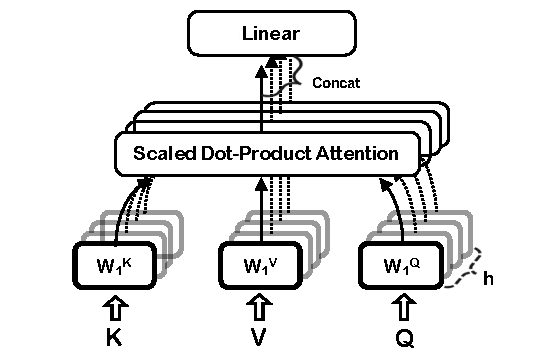
\includegraphics[width=.45\textwidth]{./images/attention.pdf}
\caption{ Illustration of Multi-Head Attention block. Each block consists of $L$ attention layers. 
}
\label{fig:multiattention}
\end{figure} 

\subsubsection{Transformer Model}
A Transformer Model is composed of a stack of identical transformer blocks, whose main component is a self-attention architecture.
It takes as input the summation of word embedding and the positional encoding offset by 1 position through a masked multi-head attention block, which prevents future words from being seen by the block. 

The transformer block consists of several consecutive linear transformations.
Let $\mathcal{H}_{\textsc{M-Att}}$ denotes the multi-head attention block, $\mathcal{H}_{\textsc{Norm}}$ be the normalization layer and $\mathcal{H}_{\textsc{FFN}}$ be the feed forward layer.
Let K, V, and Q denote the key, value, and query respectively, which are inputs to the attention block.
The transformer block can be summarized as follows:
\begin{equation}
\begin{split}
\tilde{o_1}^\ell&=\mathcal{H}_{\textsc{M-Att}}(\textrm{K}, \textrm{V}, \textrm{Q}) \\
\tilde{o_2}^\ell &= \mathcal{H}_{\textsc{Norm}}(\tilde{o_1}^\ell + \tilde{\mathbf{o}}^{\ell-1})   \\
\tilde{o_3}^\ell &= \mathcal{H}_{\textsc{FFN}}(\tilde{o_2}^\ell)   \\
\tilde{o}^{\ell}&= \mathcal{H}_{\textsc{Norm}}(\tilde{o_3}^\ell \tilde{o_2}^\ell),
\end{split}
\end{equation}
In the context of the transformer blocks used in our work, the video encoding acts as the key, the concatenation of video/caption encoding is the value, and the output from the previous transformer block acts as the query.


\subsubsection{Multi-head Attention Block}
\label{sec:att_block}
In the masked multi-head attention block, the transformer block is used with K, V, and Q being identical vectors of the input embedding.
An example of a multi-head attention block is shown in Figure~\ref{fig:multiattention}.
The motivation of the design originates from the self-attention mechanism that aims to solve the problem of long-term dependencies because of which the propagated gradients tend to vanish or explode. 
    Instead of handling sequences word by word, the self-attention block learns the attention weight between every word and produces a representation with a global view of the input.
A self-attention block with $L$ heads is formulated as: 
\begin{equation}
\mathcal{H}_{\textsc{M-Att}}(\textsc{K}, \textsc{V}, \textsc{Q}) = \mathcal{H}_{\textsc{FFN}}([{g_1}, {g_2}, ..., {g_L}]).
\end{equation}
$g_i$ for every head-index $i$ is computed by a scaled dot-product attention operation as:

\begin{equation}
{g_i} = \textsc{Softmax}\xbigg(\frac{\textsc{w}^\textsc{q}_i \textsc{Q}\cdot \textsc{w}^\textsc{k}_i \textsc{K}^\prime}{\sqrt{d_k}}\bigg)\textsc{w}^\textsc{v}_i \textsc{V}, \forall i \in \{1, \dots, L \},
\end{equation}
where $d_k$ is the dimension of keys, and $\textsc{w}_i$ are the learnable parameters of the linear transformation.

% \section{Related Literature}


In what follows, we will introduce our progress towards each perspective as stated above. In Chapter 2, we summarize our effort to build a VL grounding model from weak supervisions, achieving satisfactory grounding results compared with explicit supervised models. Furthermore, we also investigate the effort of extending the weakly-supervised grounding to videos. In Chapter 3, we then introduce a novel self-supervised visual representation learning algorithm that is facilitated by knowledge distillation technique which achieves major performance gain. We extend this contrastive learning-based distillation algorithm to the VL representation learning on a small VL architecture. Chapter 4 presents a one-stage VL model that is object detector-free and can be end-to-end optimized dubbed ViTCAP, experiment shows that our ViTCAP reaches state-of-the-art image captioning performances amongst all existing one-stage VL models. We finally summarize our work and point some future research directions in the end.